% Part 5: gravitational decoherence at the quantum level.
% Carried line by line from: Gravitational Decoherence from Dual-Sector Thermodynamics: Predictions for Optomechanical Experiments and Quantum Computing
% Architecture (Feb 2026; abstract, sections 1-10, Figs. 1-12, Table 1). The acknowledgments and repository notes are not carried.
% Corrections applied: errata GD1-GD5 (docs/verification/PAPER_ERRATA.md), docs/verification/quantum/GRAV_DECOHERENCE_CHECK.md items 1-6; silica density
% 2200 kg m^-3 throughout (book value). New findings on this read (MANIFEST_virial.md): position dephasing heats (phonon number is not conserved);
% the printed heating power equals one bit per tau_IAM, not the bit rate of the rate equation; detection forecasts rest on the earlier tau and are restated.
% Numbers: docs/verification/scripts/verify_virial_papers.py (section L, M) and verify_grav_decoherence.py; figures: fig_p5.py
% (fig_decoherence_profiles) and fig_virial_book.py (fig_gravdec_scaling, fig_gravdec_lindblad, fig_gravdec_heating).

\chapter{Gravitational decoherence at the quantum level}\label{ch:gravdec}

\section*{Overview}
This chapter investigates gravitationally induced decoherence within a semiclassical framework motivated by IAM. The analysis is formulated in the language
of open quantum systems and does not introduce objective collapse dynamics or non-unitary modifications to the Schr\"odinger equation. Instead, gravitational
interactions are treated as an environment that can suppress off-diagonal elements of the reduced density matrix through entanglement and coarse-graining.
It examines the scaling of the associated decoherence rate and its thermodynamic interpretation, with attention to energy conservation, covariance, and
existing experimental constraints. The goal is not to resolve the measurement problem, but to clarify the role of gravitational interactions in effective
classicalization processes relevant to macroscopic and cosmological systems.

\section{From cosmological to quantum scales}\label{sec:gd_scales}
\paragraph{The cosmological derivation.} At cosmological scales, IAM derives the activation function $E(a)$ through the following thermodynamic chain
(Chapter~\ref{ch:theory}). The apparent horizon of a matter-dominated universe carries Bekenstein--Hawking entropy proportional to its area. The
Gibbons--Hawking temperature provides the thermodynamic temperature of this horizon. As gravitational structure formation proceeds --- collapse,
virialization, black hole formation --- irreversible processes produce informational entropy at a rate governed by the information surface density on the
horizon. The information surface density on the apparent horizon scales as $1/a^2$ during matter domination. Integrating the cumulative decoherence rate
yields $E(a)=\exp(1-1/a)$. The coupling constant $\beta_m=\Omega_m/2=0.15765$ follows from the virial theorem (Chapter~\ref{ch:virial}). The
perturbation-level prediction is $\mu(a)=H^2_{\Lambda\rm CDM}/(H^2_{\Lambda\rm CDM}+\beta_mE(a)H_0^2)<1$ with $\Sigma(a)=1$, and $\mu_0=-0.136$, all derived
without free parameters. \derived

\paragraph{Cosmological validation.} The dual-sector framework has been tested in 18 converged Planck 2018 chains: twelve with MGCAMB (Level~1) and a baryon
test, three with the term coded directly into CAMB's matter perturbations (Level~2) and two with it in the background (Level~2b); every chain reached
$R-1\le0.01$ (Chapter~\ref{ch:dual}). In the Level~2 dual-sector perturbation chains IAM's own equations reproduce the Planck data with no added parameter, at current CMB precision
($\Delta\chi^2=+0.54$ against $\Lambda$CDM at the best points), and give $\sigma_8$ from $0.8087$ ($\Lambda$CDM) to $0.7998$, $S_8=0.822\pm0.011$, and $H_0^{(m)}=72.26$\,km\,s$^{-1}$\,Mpc$^{-1}$. \measured\ The
matter-sector rate $H_0^{(m)}=72.26$ (0.75$\sigma$ from SH0ES) and the photon-sector rate $H_0^{(\gamma)}=67.16$ (0.37$\sigma$ from Planck) place both Hubble
tension endpoints within $1\sigma$ simultaneously (Chapter~\ref{ch:virial}) \calc; the comparison of $S_8$ with each weak-lensing survey is in
Chapter~\ref{ch:sectortension}.

\paragraph{Level 2b: the background modification as a structural test.} Two Level~2b chains tested the IAM term applied to the background Friedmann equation
(modifying CAMB's \texttt{dtauda} function). These chains ran to full convergence ($R-1=0.0100$ and $0.0068$). The converged result was
$H_0=61.45\pm0.42$ and $61.52\pm0.43$\,km\,s$^{-1}$\,Mpc$^{-1}$ --- far from the Planck value of 67.4. \measured\ This is a structural result: when the
dual-sector modification is applied to the background expansion rather than the perturbation equations, the global expansion rate shifts far from every
measurement. The standard $\Lambda$CDM Friedmann equation correctly describes the global background. The dual-sector mechanism lives exclusively in the
perturbation equations, entering through the expansion rate felt by matter perturbations and leaving the background untouched (Chapter~\ref{ch:level2}). \interp
All chains are archived for full reproducibility.

\paragraph{The quantum analogue.} The sector split follows from causal structure: massive particles on timelike worldlines ($\Delta\tau>0$) pay
gravitational Landauer cost; photons on null geodesics ($\Delta\tau=0$) do not. At cosmological scales, the boundary is the apparent horizon. At quantum
scales, the boundary is proposed to be the spatial extent of the quantum superposition. \conjecture

\section{Di\'osi--Penrose and the IAM rate}\label{sec:gd_rate}
Di\'osi~\cite{Diosi1987,Diosi1989} and Penrose~\cite{Penrose1996} proposed that a superposition of two mass distributions separated by more than their size
decays on the timescale
\begin{equation}
 \tau_{\mathrm{DP}}\simeq\frac{\hbar}{E_G},\qquad E_G\simeq\frac{Gm^2}{R},\label{eq:gd_dp}
\end{equation}
with $E_G$ the gravitational self-energy of the difference of the mass distributions, here for a uniform sphere of mass $m$ and radius $R$. The prediction
is temperature-independent. For one class of mass distributions it has been constrained by underground radiation measurements~\cite{Donadi2021}. Levitated
optomechanics is approaching the regime needed to test it directly~\cite{RomeroIsart2011,Gonzalez2021,Delic2020,Neumeier2024,Rossi2025}, and space missions
have been proposed for it~\cite{Kaltenbaek2012}. \observed

IAM modifies this through Landauer's principle~\cite{Landauer1961}: erasing one bit requires minimum dissipation $Q_L=k_BT\ln2$, a bound now tested in the
laboratory, including with levitated optomechanics~\cite{Berut2012,Ciampini2025}. IAM takes the rate of information production to be
\begin{equation}
 \frac{dN_{\mathrm{bits}}}{dt}=\frac{E_G^2}{\hbar\,\kB T\ln2},\label{eq:gd_bitrate}
\end{equation}
and the information capacity of the superposition boundary to be $S_{\mathrm{boundary}}=\kB T/E_G$. Both are taken as given here; deriving them from the law is an open problem.
\conjecture{} The temperature dependence that follows runs opposite to every known environmental decoherence, which strengthens with temperature; that is
what makes it testable, and it is the most exposed claim of the chapter. Following the cosmological derivation, the cumulative integral is
\begin{equation}
 \ln E_q(t)=\int_0^t\frac{\Gamma_{\mathrm{info}}(t')}{S_{\mathrm{boundary}}}\,dt'=\frac{E_G^3}{\hbar\,\kB^2T^2\ln2}\,t,\qquad
 \boxed{\;\tau_{\mathrm{IAM}}=\frac{\hbar\,\kB^2T^2\ln2}{E_G^3}\;}
 \label{eq:tauIAM}
\end{equation}
The integrand is constant, so the integral gives a plain exponential with time constant $\tau_{\mathrm{IAM}}$. \derived\ (sympy: \texttt{verify\_virial\_papers.py}
section L.) Defining $\eta=t/\tau_{\rm IAM}$, an alternative carries over the functional form of the cosmic activation function,
\begin{equation}
 E_q(\eta)=\exp\!\left(1-\frac1\eta\right),\qquad C_{\mathrm{IAM}}(t)=1-\frac{E_q(t/\tau_{\mathrm{IAM}})}{e},\label{eq:gd_ramp}
\end{equation}
formally identical to the cosmological $E(a)$, in place of the exponential $C_{\mathrm{DP}}(t)=\exp(-t/\tau_{\mathrm{DP}})$. It is an assumption, separate from the integral above: the cosmological ramp comes from the $1/a^2$ surface density on the horizon, and deriving its analogue at the superposition boundary is the open step. \conjecture\ \openprob

\begin{figure}[htbp]\centering
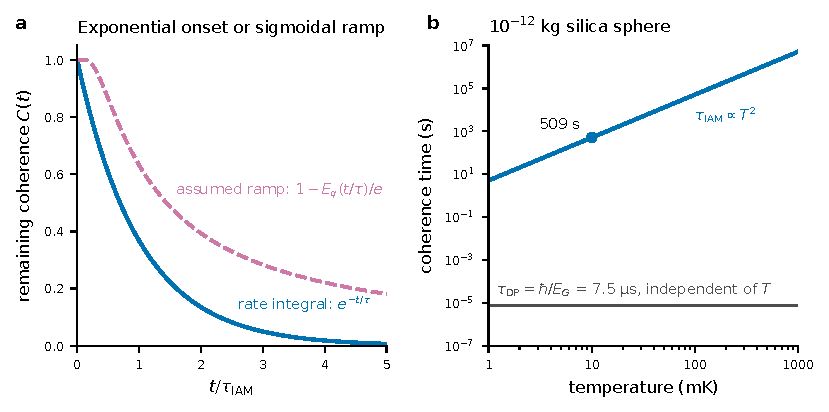
\includegraphics[width=\textwidth]{figures/part4/fig_decoherence_profiles.pdf}
\caption{(a) Remaining coherence against $t/\tau_{\rm IAM}$: the plain exponential the rate integral gives, and the ramp $1-E_q(t/\tau)/e$, $E_q(\eta)=\exp(1-1/\eta)$, carried over from the cosmology \conjecture. (b) $\tau_{\rm IAM}$ against temperature for a $10^{-12}$\,kg silica sphere ($\rho=2200$\,kg\,m$^{-3}$, $R=4.8\,\mu$m, $E_G=1.4\times10^{-29}$\,J): 509\,s at 10\,mK, growing as $T^2$ (factors 4 and 16 at 20 and 40\,mK), against the temperature-independent $\tau_{\rm DP}=7.5\,\mu$s. \prediction}\label{fig:decoherence_profiles}
\end{figure}
For a $10^{-12}$\,kg nanosphere at 10\,mK, $\tau_{\rm IAM}=509$\,s. \calc\ Under the ramp the rate of loss of coherence is zero at $t=0$ --- a protected
regime --- and peaks at $\eta=1/2$, while the Di\'osi--Penrose rate is largest at $t=0$ (Figure~\ref{fig:gd_scaling}b). If the ramp held, this qualitative
difference at early times would be the primary experimental discriminator, accessible without high-precision measurements. \conjecture

\section{Quantitative predictions}\label{sec:gd_predictions}

\begin{figure}[htbp]\centering
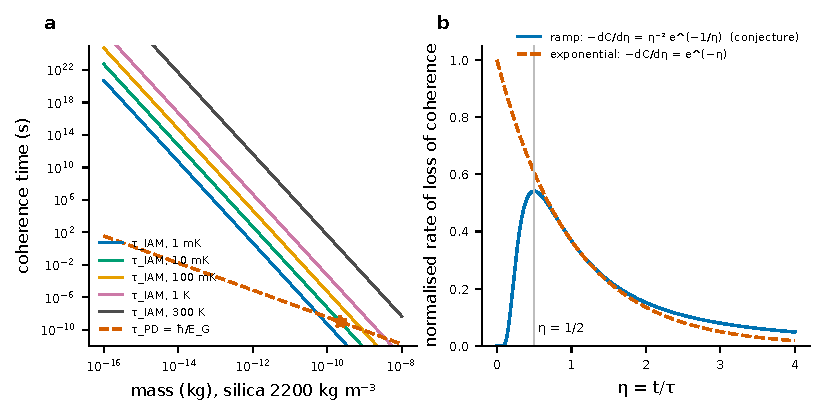
\includegraphics[width=\textwidth]{figures/part4/fig_gravdec_scaling.pdf}
\caption{(a) $\tau_{\rm IAM}$ against mass for silica spheres ($\rho=2200$\,kg\,m$^{-3}$) at five temperatures, 1\,mK to 300\,K, against $\tau_{\rm PD}=\hbar/E_G$ (dashed; no temperature dependence). At 10\,mK the two cross at $2.2\times10^{-10}$\,kg (star). \prediction\ (b) Normalised rate of loss of coherence, $-dC/d\eta$: the ramp $\eta^{-2}e^{-1/\eta}$, zero at $t=0$ with its peak at $\eta=1/2$ \conjecture, and the exponential $e^{-\eta}$. \calc}\label{fig:gd_scaling}
\end{figure}

\paragraph{Timescales across mass scales.} Figure~\ref{fig:gd_scaling}a shows $\tau_{\rm IAM}$ against mass from dust grains down to the mesoscopic range at
five temperatures, compared against Di\'osi--Penrose. At fixed density $\tau_{\rm IAM}\propto m^{-5}$: at 10\,mK it is $5\times10^{17}$\,s at $10^{-15}$\,kg,
509\,s at $10^{-12}$\,kg and $5\times10^{-8}$\,s at $10^{-10}$\,kg; it falls below 1\,s only above $3.5\times10^{-12}$\,kg and below 1\,ms above
$1.4\times10^{-11}$\,kg. \calc\ The mass range where IAM predictions become testable with coherence times of milliseconds to seconds is therefore
$10^{-12}$--$10^{-11}$\,kg at dilution-refrigerator temperatures. The $T^2$ temperature dependence of IAM separates the coloured curves; Di\'osi--Penrose
produces a single curve.

\paragraph{Temperature dependence: the key discriminator.} $\tau_{\rm IAM}\propto T^2$ for a fixed nanosphere mass (Figure~\ref{fig:decoherence_profiles}b).
Running the same experiment at 10, 20 and 40\,mK produces a factor of 4 and 16 increase in $\tau_{\rm IAM}$ respectively. \calc\ Di\'osi--Penrose predicts
no change. This is the single cleanest test: doubling the temperature produces a $4\times$ longer coherence time under IAM.

\paragraph{Mass scaling in the mesoscopic regime.} At fixed density $E_G\propto m^{5/3}$, so $\tau_{\rm IAM}\propto E_G^{-3}\propto m^{-5}$, against
$\tau_{\rm PD}\propto m^{-5/3}$; the difference in power-law exponent is $\Delta\alpha=10/3=3.33$. \calc\ The crossover occurs near $m\approx2.2\times10^{-10}$\,kg
at 10\,mK. Below the crossover, IAM predicts slower decoherence; above it, faster. Measuring $\tau$ at 3--4 bead masses spanning one order of magnitude with
10\,\% precision on each discriminates between log slopes of $-5$ and $-5/3$ at well over $5\sigma$ (four masses equally spaced in $\ln m$ over a decade give
$\sigma(\alpha)\approx0.06$). \calc

\paragraph{Landauer heating rate.} Each bit written at the boundary costs at least $k_BT\ln2$. One bit per decoherence time gives the dissipated power and,
for a mode of frequency $\omega_0$, the phonon excitation rate
\begin{equation}
P_{\rm IAM}=\frac{k_BT\ln2}{\tau_{\rm IAM}}=\frac{E_G^3}{\hbar\,k_BT},\qquad\frac{dn}{dt}=\frac{E_G^3}{\hbar^2k_BT\,\omega_0}.\label{eq:gd_heating}
\end{equation}
\calc\ $P_{\rm IAM}\propto1/T$: colder systems dissipate more power. This is the inverse of environmental heating ($P_{\rm env}\propto T$). For
$10^{-12}$\,kg at 10\,mK, $P_{\rm IAM}=1.9\times10^{-28}$\,W and $dn/dt=2.8$ phonons\,s$^{-1}$ at $\omega_0=2\pi\times100$\,kHz; the rate passes
1\,phonon\,s$^{-1}$ at $0.8\times10^{-12}$\,kg and grows as $m^5$ (Figure~\ref{fig:gd_heating}). \calc\ The bit rate of Eq.~\eqref{eq:gd_bitrate} priced at
$k_BT\ln2$ would instead give $E_G^2/\hbar=1.9\times10^{-24}$\,W; which of the two counts the energy actually dissipated is an open problem, pending derivation of the rate and the boundary capacity. \openprob

\begin{figure}[htbp]\centering
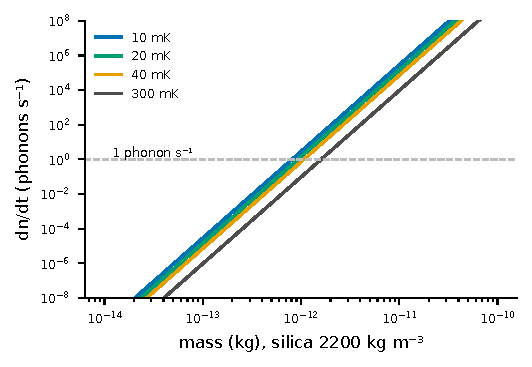
\includegraphics[width=0.6\textwidth]{figures/part4/fig_gravdec_heating.pdf}
\caption{Phonon excitation rate $dn/dt=E_G^3/(\hbar^2k_BT\omega_0)$ of Eq.~\eqref{eq:gd_heating} against mass at four temperatures (silica, $\omega_0=2\pi\times100$\,kHz). Dashed: 1\,phonon\,s$^{-1}$. Colder systems give the larger signal. \prediction\ \conjecture}\label{fig:gd_heating}
\end{figure}

\section{Lindblad dynamics with a time-dependent rate}\label{sec:gd_lindblad}
If the ramp of Eq.~\eqref{eq:gd_ramp} holds, it implies a time-dependent Lindblad decoherence rate~\cite{Lindblad1976},
\begin{equation}
\Gamma_{\rm IAM}(\eta)=\frac{dE_q}{d\eta}=\frac{1}{\eta^2}\exp\!\left(1-\frac1\eta\right),\qquad\eta=t/\tau_{\rm IAM},\label{eq:gd_gamma}
\end{equation}
and the density matrix evolves under
\begin{equation}
\frac{d\rho}{d\eta}=\Gamma(\eta)\left(L\rho L^\dagger-\tfrac12\{L^\dagger L,\rho\}\right),\label{eq:gd_lindblad}
\end{equation}
where the collapse operator $L\propto\hat x$ (position) implements gravitational dephasing: spatial coherence decays. \conjecture\ Position dephasing does not
conserve energy: it diffuses momentum, and with $L=\hat x$ in units of the zero-point width $\langle n\rangle$ grows at $\Gamma/2$ per unit $\eta$ for any
state. \derived\ The integrated rate $\int_0^\eta\Gamma\,d\eta'=E_q(\eta)$ equals the constant-rate value $\eta$ at $\eta=1$.

\begin{figure}[htbp]\centering
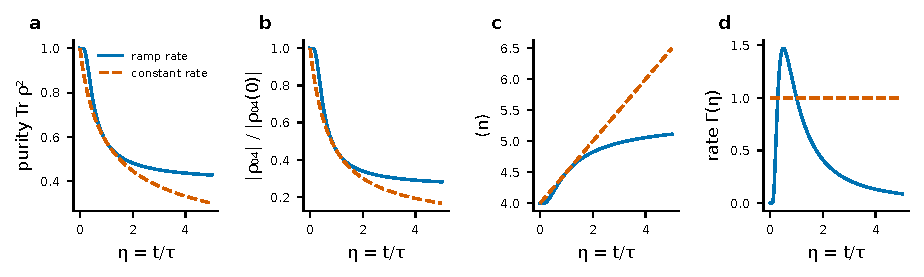
\includegraphics[width=\textwidth]{figures/part4/fig_gravdec_lindblad.pdf}
\caption{Dephasing of an initial coherent state $|\alpha=2\rangle$ under Eq.~\eqref{eq:gd_lindblad} with $L=\hat x=(a+a^\dagger)/\sqrt2$, the oscillator Hamiltonian neglected (dephasing in a frame rotating with the oscillator is not modelled), fourth-order Runge--Kutta in a 40-state Fock basis. Solid: the ramp rate of Eq.~\eqref{eq:gd_gamma}; dashed: a constant rate $\Gamma=1$. (a) Purity ${\rm Tr}\rho^2$. (b) The coherence $|\rho_{04}|$ normalised to its initial value. (c) Mean phonon number $\langle n\rangle$, which grows: position dephasing heats. (d) The rate. The purity difference peaks at $\eta=0.225$, $\Delta P=0.139$. \calc\ (under the ramp \conjecture)}\label{fig:gd_lindblad}
\end{figure}

\paragraph{Quantum state evolution.} Figure~\ref{fig:gd_lindblad} shows the evolution of an initial coherent state $|\alpha=2\rangle$ under the ramp and
under a constant rate (standard Lindblad decoherence). Under the ramp the purity stays higher in the protected regime ($\eta<0.5$), entropy production has a
delayed onset, and the off-diagonal coherence is preserved longer at early times; the ramp rate is zero at $t=0$ and peaks at $\eta=0.5$, while the standard
rate is constant. The purity is $0.759$ against $0.707$ at $\eta=0.5$, equal ($0.577$) at $\eta=1$, and $0.482$ against $0.447$ at $\eta=2$; at $\eta=5$ it is
$0.43$ against $0.30$, both states close to diagonal. \calc

\paragraph{Information thermodynamics.} The purity difference $\Delta P=P_{\rm IAM}-P_{\rm std}$ peaks at $\eta\approx0.225$ ($\Delta P\approx0.14$). \calc\
This is the observable quantity and, if the ramp holds, the optimal measurement time for discriminating it from standard Lindblad decoherence. It is not the
peak of the rate, which lies at $\eta=0.5$. The mean phonon number rises under both rates and is lower under the ramp at every $\eta$ except $\eta=1$, where the two are equal, since $E_q(\eta)\le\eta$. \derived

\section{Detection}\label{sec:gd_detection}
\paragraph{Profile shape.} An experiment measuring coherence $C(t)$ at $N=50$ time points with $\sigma_C=2\,\%$ precision at 10\,mK separates the ramp from an
exponential with the same $\tau$ at high significance once $\tau_{\rm IAM}$ falls within the time over which the superposition can be held. With the
decoherence time of Eq.~\eqref{eq:tauIAM} this requires masses near or above $10^{-12}$\,kg (509\,s) and, for sub-second coherence, above
$3.5\times10^{-12}$\,kg at 10\,mK. \calc\ Below the crossover at $2.2\times10^{-10}$\,kg the Di\'osi--Penrose time is the shorter of the two: there the models
are distinguished by which one is seen at all, not by their profile shapes.

\paragraph{Temperature and mass scaling.} Three temperatures (10, 20, 40\,mK) test $\tau\propto T^2$ against a constant $\tau$: the factor of 16 between the
ends is a $9.8\sigma$ separation from a constant $\tau$ with 20\,\% precision on each $\tau$. Four masses spanning one decade test $m^{-5}$ against $m^{-5/3}$. Both tests are
sensitive wherever $\tau_{\rm IAM}$ is measurable, $10^{-12}$--$10^{-11}$\,kg at 10\,mK. \calc

\paragraph{Phonon heating.} The anomalous IAM phonon excitation rate rises as temperature falls, the direct consequence of $P_{\rm IAM}\propto1/T$, and passes
the present optomechanical sensitivity of about 1\,phonon\,s$^{-1}$ near $10^{-12}$\,kg (a nanogram) at dilution-refrigerator temperatures
(Figure~\ref{fig:gd_heating}). \prediction\ A signal that grows on cooling cannot be mimicked by thermal noise.

\paragraph{Timeline.} The mass held under quantum control has advanced by roughly a factor of ten every three to five years; that trend is an estimate,
not a law. \calc\ Starting from nanoparticle quantum control (delocalisation) at $10^{-19}$\,kg~\cite{Rossi2025,Neumeier2024}, the $3.5\times10^{-12}$\,kg
at which $\tau_{\rm IAM}$ reaches one second at 10\,mK lies seven and a half decades higher: about 23--38 years if the trend holds. \calc\ The heating signature near a nanogram needs no spatial superposition of that size and is
the nearer test. The cosmological test of the same framework, the growth of structure measured by Euclid and DESI, comes first
(Chapter~\ref{ch:virial_tests}).

\section{Comparison with Di\'osi--Penrose}\label{sec:gd_compare}
The IAM law differs from Di\'osi--Penrose in four ways, each testable (Table~\ref{tab:gd_compare}):
\begin{enumerate}
 \item \textbf{Temperature.} $\tau_{\mathrm{IAM}}\propto T^2$: a \emph{hotter} object stays coherent \emph{longer}. The Di\'osi--Penrose time is independent
       of $T$. Running at 10, 20 and 40~mK should lengthen $\tau$ by factors of 4 and 16.
 \item \textbf{Mass.} $\tau_{\mathrm{IAM}}\propto E_G^{-3}\propto m^{-6}R^3$, against $\tau_{\mathrm{DP}}\propto m^{-2}R$ (at fixed density,
       $\tau_{\mathrm{IAM}}\propto m^{-5}$ and $\tau_{\mathrm{DP}}\propto m^{-5/3}$).
 \item \textbf{Heating.} $P_{\rm IAM}\propto1/T$, against no heating for Di\'osi--Penrose.
 \item \textbf{Profile (only if the assumed ramp holds).} $C(t)$ would have zero slope at $t=0$ and a sigmoidal onset; the rate integral gives an exponential.
       A measured exponential onset with the $T^2$ and mass scalings would support the rate and reject the ramp.
\end{enumerate}

\begin{table}[htbp]\centering\small
\caption{IAM against Di\'osi--Penrose. The IAM entries follow from Eqs.~\eqref{eq:tauIAM} and~\eqref{eq:gd_heating} \calc; the ramp is \conjecture.}\label{tab:gd_compare}
\begin{adjustbox}{max width=\textwidth}
\begin{tabular}{lllll}
\hline
Model & Profile & $T$ scaling of $\tau$ & Mass scaling (fixed density) & Heating\\\hline
IAM & exponential (ramp if Eq.~\eqref{eq:gd_ramp} holds) & $T^2$ & $m^{-5}$ & $P\propto1/T$\\
Di\'osi--Penrose & exponential & none & $m^{-5/3}$ & none\\\hline
\end{tabular}
\end{adjustbox}
\end{table}
The comparison with continuous spontaneous localisation, graviton-emission and semiclassical-gravity decoherence is to be made against their published rate
formulas for the same silica spheres. \openprob

\begin{checkbox}[title={Independent check: the numbers}]
\textbf{Dimensions.} $\hbar\kB^2T^2/E_G^3$ has units $\mathrm{J\,s}\cdot\mathrm{J}^2/\mathrm{J}^3=\mathrm s$.
Correct.

\textbf{The cat.} $m=4$~kg, $E_G=7.1\times10^{-9}$~J (implying $R\approx0.15$~m), $T=300$~K:
Eq.~\eqref{eq:tauIAM} gives $3.5\times10^{-51}$~s. \calc{} Environmental decoherence of a warm macroscopic body is faster still, so the number illustrates the formula; it is not the
mechanism that makes a cat classical.

\textbf{The nanosphere.} For a $10^{-12}$~kg silica sphere ($\rho=2200\ \mathrm{kg\,m^{-3}}$,
$R=4.8\ \mu$m), $E_G=1.4\times10^{-29}$~J, and Eq.~\eqref{eq:tauIAM} gives $\tau_{\mathrm{IAM}}=509$~s
at 10~mK, against $\tau_{\mathrm{DP}}=7.5\ \mu$s. \calc{} At physical densities the IAM time for a
$10^{-12}$~kg sphere is about $7\times10^{7}$ times the Di\'osi--Penrose time, so the two models are
distinguished by \emph{which one is seen at all}, not by their profile shapes.
\end{checkbox}

\section{Implications for quantum computing}\label{sec:gd_qc}
\paragraph{Current architectures and the gravitational floor.} Gravitational decoherence is irrelevant for all current quantum computing platforms.
Superconducting qubits (effective moving mass $\sim10^{-20}$\,kg), trapped ions ($\sim10^{-25}$\,kg), and photonic systems ($E_G=0$) all have $\tau_{\rm IAM}$
and $\tau_{\rm DP}$ far exceeding any practical timescale. \calc{} IAM does not predict that current quantum computers will fail. Their decoherence is
electromagnetic and material, which is where Part~\ref{part:3} reads them.

IAM does identify an engineering target distinct from isolation. The isolation paradigm: decoherence is noise, so engineer silence --- move to the Moon. The
IAM paradigm: decoherence is irreversible information production, so engineer reversibility and design better gates on Earth. As environmental isolation
improves, residual decoherence will increasingly be dominated by irreversible thermodynamic interactions in gate operations; at that point further
isolation provides diminishing returns. \interp

\paragraph{Five principles.} \interp
\begin{enumerate}
\item \emph{Work with the ramp.} If the ramp holds, design computations that complete within $t<0.5\,\tau_{\rm IAM}$, where the decoherence rate is near zero.
\conjecture
\item \emph{Minimize irreversible interaction.} Only irreversible interactions ($Q\ge k_BT\ln2$) advance the record; reversible interactions do not contribute
to gravitational decoherence.
\item \emph{The $\Sigma=1$ principle.} Photons have $E_G=0$ and $\tau_{\rm IAM}=\infty$. Photonic qubits are immune to gravitational decoherence by the causal
structure of spacetime, not by engineering.
\item \emph{The feedback loop as resource.} When a qubit decoheres, information is encoded rather than destroyed. Instrumenting the environment to capture
this encoding would enable computation through controlled decoherence. \conjecture
\item \emph{The Landauer floor as constraint.} The minimum energy cost per irreversible operation is $k_BT\ln2$; operate as close to this floor as possible.
\end{enumerate}

\section{Where the two sectors meet}\label{sec:gd_sectors}
In the dual-sector picture, the matter sector ($\mu<1$) decoheres gravitationally and the photon sector ($\Sigma=1$) does not. \conjecture\ Trapped ions
($m\sim10^{-25}$~kg) and superconducting qubits (effective moving mass $\sim10^{-20}$~kg) have $\tau_{\mathrm{IAM}}$ and $\tau_{\mathrm{DP}}$ both far beyond
any practical time.

The decoherence rate $E_G^3/(\hbar k_B^2T^2\ln2)$ at laboratory scales is proposed to be the same physical process that, accumulated over $\sim10^{11}$
galaxies and 13.8\,Gyr, produces the informational entropy that modifies the growth of cosmic structure. The laboratory measures the rate per event;
cosmology measures the cumulative effect. At cosmological scales, $E(a)=\exp(1-1/a)$ modifies the matter-sector perturbation equations and produces $\mu<1$,
$\Sigma=1$. At quantum scales the same functional form, $E_q(\eta)=\exp(1-1/\eta)$, is proposed for the decoherence profile of individual mesoscopic
systems. \conjecture\ Simultaneous positive results --- Euclid detecting $\mu<1$ and optomechanical experiments measuring the predicted $\tau_{\rm IAM}$ with
its $T^2$ law --- would close the loop from quantum decoherence to cosmic structure.

\section{Falsification criteria}\label{sec:gd_falsify}
IAM's quantum-scale predictions are falsified if:
\begin{enumerate}
\item No gravitational decoherence is detected at masses where $\tau_{\rm IAM}$ is shorter than the coherence time held (above about
$3.5\times10^{-12}$\,kg for one second at 10\,mK), with environmental decoherence controlled below the IAM-predicted rate.
\item The mass scaling exponent is inconsistent with $\alpha=5$ (IAM, fixed density); a measured $5/3$ would favour Di\'osi--Penrose.
\item The temperature dependence is inconsistent with $T^2$.
\item Coherence times exceed $\tau_{\rm IAM}$ for a given mass.
\item For the ramp alone: the decoherence profile is exponential, not the $E_q$ ramp. This would reject Eq.~\eqref{eq:gd_ramp} and leave
Eq.~\eqref{eq:tauIAM} standing.
\end{enumerate}
Falsification of the quantum predictions would not automatically falsify the cosmological predictions ($\mu<1$, $\Sigma=1$), which could arise from a
different microscopic mechanism with the same macroscopic consequences. The two test regimes are complementary: cosmology tests the cumulative effect; the
laboratory tests the underlying cause.

\section{Conclusion}\label{sec:gd_conclusion}
The IAM decoherence timescale $\tau_{\rm IAM}=\hbar k_B^2T^2\ln2/E_G^3$ contains no free parameters once the boundary capacity $k_BT/E_G$ is assumed, and it
produces three experimental signatures that separate it from Di\'osi--Penrose: $\tau\propto T^2$, $\tau\propto m^{-5}$ at fixed density, and heating that
grows on cooling. \prediction\ The quantum analogue $E_q(\eta)=\exp(1-1/\eta)$ of the cosmological activation function $E(a)=\exp(1-1/a)$ would add a fourth,
the ramp profile; modified Lindblad dynamics under the time-dependent $E_q$ rate then show a measurable purity difference peaking at $\eta\approx0.225$, the
optimal discrimination time. \conjecture\ The rate and the boundary capacity are taken as given here; their derivation at the superposition boundary is an open problem.
\openprob

The temperature and mass scalings here are stated plainly enough for an optomechanics group to check against a running apparatus. A relativist can take up the derivation at the superposition boundary; an experimentalist can look for the signature. Either one moves the open problem forward.

The missing piece was always information.
